\section{Evaluation}
\label{sec:eval}

Every measurement here is on A100/PCIe, which \S\ref{sec:model:omits} predicts
cannot pay. So this section establishes the mechanism, the cost structure and the
model's \emph{negative} predictions, and states the two questions it cannot close
--- whether the model's positive prediction holds, and whether a second tier
raises \emph{goodput} rather than raw throughput --- as protocols with predictions
attached. Each subsection opens with its question, the claim under test, and what
the model predicts, before any number.

\subsection{Setup}
\label{sec:eval:setup}

\paragraph{Hardware.} A100-80 over PCIe~4. What rules PCIe out is not the latency
gate of \S\ref{sec:model:gate}, which contains no $\Xlink$ and so says nothing about
an interconnect, but the bandwidth crossover and fixed cost of
\S\ref{sec:model:omits}; a GH200-96 over NVLink-C2C is the substrate the positive
claims require, and those experiments are in progress. We measure the PCIe link at
$25.1$\,GB/s for the per-layer bulk copy, falling to $0.52$ at 4\,KB granularity,
which is why the transfer path issues runs rather than blocks
(\S\ref{sec:impl:pool}).
% src: paper/model/transfer_bw_a100.json @ 2bfc6ca5e For C2C we use
an \emph{independent} measurement of the same part, $419$\,GB/s
host-to-device~\cite{pie}, rather than the widely cited 900\,GB/s, which is
bidirectional where a KV stream is not; we have not measured C2C.

\paragraph{Method.} Every absolute is taken on an idle, exclusively allocated device
--- the same measurement on a contended node differed by $9.4\times$
(Appendix~\ref{app:impl}) --- from a fixed-context, fixed-output, closed-loop run at
2048 context and 64 output tokens, with offered load and resident cohort stated per
experiment. That shape isolates a host-tier request's cost and is the wrong shape for
goodput, which is why \S\ref{sec:eval:goodput} is a protocol. The baseline is stock
vLLM with tiering disabled, matching the unmodified engine to within $0.08\%$ across
six interleaved runs (Appendix~\ref{app:setup}).
% src: paper/data/baseline_integrity_20260912.log @ 5377be7c3
Appendix~\ref{app:setup} gives the models, the pools, the metric definitions and
the comparability rules for the arms.

\subsection{Does the mechanism work? Are host-tier requests additive?}
\label{sec:eval:capacity}

\emph{Question.} Does admitting a host-tier request consume device blocks?
\emph{Claim under test.} That it does not, so the host cohort adds to the resident
cohort rather than displacing it --- the property Table~\ref{tab:endpoints}'s
interior point depends on. \emph{Prediction.} Concurrency rises past the all-HBM
capacity of the same pool, without the device pool growing.

Against a fixed KV pool, host-tier requests raise peak concurrency from 8 to 48,
and 48 is a lower bound because it was the entire offered load. \textbf{Both arms
completed all 48 requests, and the mixture took $89.7$\,s against the all-HBM
arm's $47.8$\,s} --- $0.53\times$ the throughput for identical work, with 42
reclaims.
% src: paper/data/preload_capacity.json @ f3df05bdb
This is a \textbf{mechanism check and not a performance result}, and three things
bound what it shows: KV is delivered synthetically, so the generated tokens are not
meaningful; no latency target is applied and none is met, since the admission
roofline of \S\ref{sec:design:admission} permits two host-tier requests at this
context, so serving 48 implies step times far outside any SLO; and the pool is
deliberately small, the same device-shrinking we criticise elsewhere, justified only
because the quantity under test is whether admission touches the pool at all. What
it establishes is that zero-block admission decouples the host cohort from the
device pool; whether that decoupling pays is \S\ref{sec:eval:cost}.

It also isolates why the system model matters. An earlier design capped a host-tier
request's block \emph{growth} while leaving its prefill resident: it freed about
11\% of the footprint while still paying full interconnect every step, and the
served total crept toward the all-HBM capacity from below without ever passing it,
at any resident cap. A request whose prefill stays resident is strictly worse than
one left in device memory, at any link speed --- which makes the disaggregated
decode-node assumption (\S\ref{sec:background:pd}) load-bearing rather than
convenient.

\subsection{Is the placement policy load-bearing?}
\label{sec:eval:ablation}

If uniform offloading at the same interconnect budget performs as well, the policy
is decoration and the contribution reduces to the analysis. The arms add one
mechanism each: uniform offload at a matched byte budget, our admission controller
choosing how many while arrival order chooses which, scored placement, and
migration.

\textbf{Matched bytes, not matched request count.} Capping how many requests are
host-tier does not control this comparison: the policies select requests of
different context lengths and so move different volume, and part of any difference
would be a difference in offload ratio wearing the appearance of a policy win. We
count bytes in both directions per arm and treat arms differing by more than
$1.25\times$ in traffic as not comparable. A parallel control matches the
resident-cohort cap, since an arm with a different cap is a different
\emph{allocation} rather than a different policy --- on A100 that distinction
accounted for most of an apparent 14.5\% difference.

The adaptive probe of \S\ref{sec:design:migration} is implemented but not reported,
for the reason that blocks the ablation: its verdict compares goodput before and
after a demotion, and where the budget admits two host-tier requests a demotion
moves one of them, so the change is inside the noise the probe's own margin absorbs.
We state its prediction instead --- revert on PCIe, keep on a coherent link. If it
keeps on PCIe or reverts on C2C, the model is wrong about which term dominates, and
that is the finding we would report.

\subsection{What a host-tier request costs}
\label{sec:eval:cost}

\emph{Question.} What does one host-tier request add to a decode step?
\emph{Claim under test.} That the cost is a transfer partly hidden behind
compute, plus a fixed per-step overhead. \emph{Prediction.} Both terms are
non-zero, and the second does not shrink with the link.

We measure this with a fixed resident batch of 16 and riders on top, taking step time
by differencing two generation lengths so prefill cancels by construction. Every
point is gated per step on decode purity --- no prefill tokens, nothing queued, and
the admitted tier counts matching the request exactly --- and a point failing the
gate is discarded rather than adjusted. The two-rider table below predates that
discipline: it is a single unreplicated comparison transcribed from a run whose
machine-readable output was not archived, and Appendix~\ref{app:ridercost} says why
the four-point sweep that accompanied it is set aside.
%
\begin{center}\small
\begin{tabular}{rrrr}
\toprule
riders & step (ms) & GB/step & growth \\
\midrule
0 & 54.10 & 0.000 & --- \\
2 & 70.79 & 1.115 & 0.62 \\
\bottomrule
\end{tabular}
\end{center}
% src: paper/data/rider_cost_4p2b.json @ 21ea9b18d
%
At that cost the marginal test fails: $\Delta T/T = 0.236$ against a threshold
of $1/(N{+}r) = 0.056$, and decode throughput --- derived as $B/\mathrm{ITL}$
from the step times, not measured end to end --- is $254$ tok/s against $296$ at
$r{=}0$. \textbf{The A100 does not show the benefit}, and the reason is the knee
rather than the per-rider price. At $25.1$\,GB/s, $r^{*} = 2.4$: the link admits two
riders, and two riders on sixteen residents cannot outrun the fixed cost. Earlier
drafts derived a crossover bandwidth of $60$\,GB/s by setting the \emph{unhidden
transfer} equal to what freed capacity buys; we withdraw that derivation, because
below the knee no part of the transfer is unhidden and the quantity it balanced does
not exist. The conclusion is unchanged and now rests on Eq.~\ref{eq:knee}. An
earlier $+7.7\%$ on the decode phase was an artifact of subtracting prefill by hand
from a co-located run, and we withdraw that too.

\begin{figure*}[t]
\centering
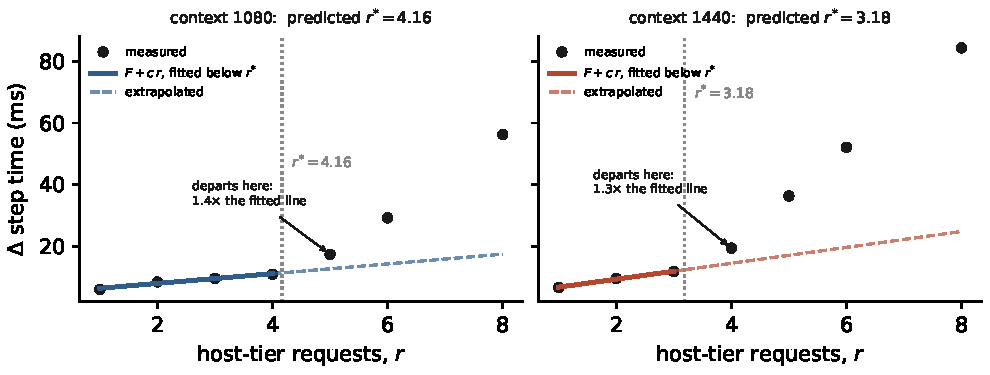
\includegraphics[width=0.49\textwidth]{figs/f8.pdf}\hfill
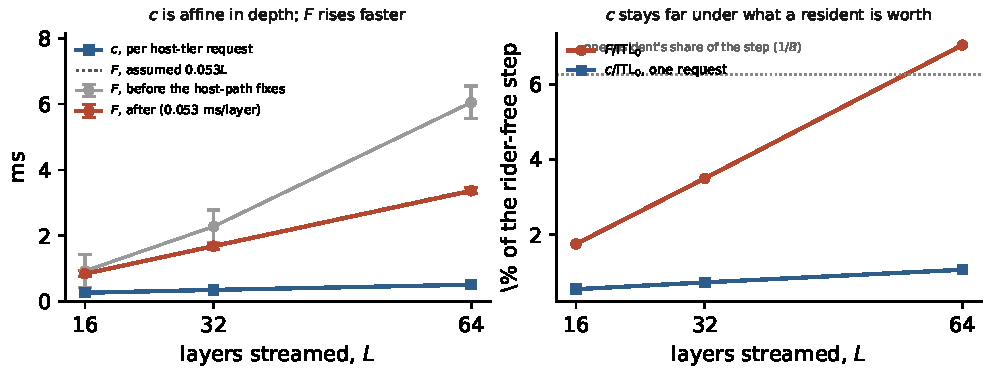
\includegraphics[width=0.49\textwidth]{figs/f7.pdf}
\caption{\textbf{Left: the governing variable is the transfer-exposure ratio, and
the boundary is at unity.} Plotting step growth against
$\ell/\mathrm{ITL}_0$ --- the transfer one request demands per step, over the
rider-free step --- collapses \emph{two different contexts onto one curve}: matched
at equal $\ell/\mathrm{ITL}_0$ the two series agree to $2$--$10\%$ across the whole
range, and both depart from linearity at $\ell/\mathrm{ITL}_0 = 1$, where the
transfer stops fitting inside the step. The knee of Eq.~\ref{eq:knee} is then a
corollary rather than a fitted quantity, $r^{*} = \lfloor \mathrm{ITL}_0/\ell
\rfloor$, which is $4$ at context 1080 and $3$ at 1440. Measured on A100/PCIe,
purity-gated, 3 repeats, resident batch 8; no projection enters this panel. It is
also the cleanest statement of why fitting a single line across the boundary
produced a \emph{negative} fixed cost: the two sides have different slopes by
construction.
\textbf{Right: $c$ is affine in depth; $F$ is not, and that matters.} $c$ tracks
Eq.~\ref{eq:coeffs} closely --- $0.263$ and $0.350$ measured against $0.263$ and
$0.350$ predicted at $L = 16$ and $32$. $F$ does not: on the same arms $F/L$ runs
$0.058$, $0.071$, $0.095$, \emph{rising} by $64\%$ across the sweep, against the flat
$0.053$ the dotted line assumes. That assumption was obtained by dividing one
depth's measurement by its depth, and Table~\ref{tab:gain} charges it at $L = 80$,
so \S\ref{sec:eval:sens} carries the consequence rather than hiding it. $F$'s bars
are its \emph{measured} between-job drift, not a fit residual.
The right panel's dotted line is what one resident request is worth, $\mathrm{ITL}_0/B$
--- $c$ stays far beneath it at every depth, which is why the per-request term is
not what decides the margin.}
% src: paper/data/overhead/21_fusion_bound/E3_ctx1080.json,
% paper/data/overhead/21_fusion_bound/E3_ctx1440.json,
% paper/data/overhead/15_clean_cf/CF_L16.json,
% paper/data/overhead/15_clean_cf/CF_L32.json,
% paper/figs/f8_knee.py, paper/figs/f7_coefficients.py
\label{fig:coeffs}
\end{figure*}

\paragraph{The law is affine, and our first reading of it was not.}
We previously reported this cost curve as \textbf{not affine} --- $\Delta T$ per
rider \emph{rising} through $9.1$, $11.0$, $15.6$\,ms at $r = 2, 4, 6$, so that
$\Delta T = F + cr$ fitted a \emph{negative} fixed cost and the split was not a
meaningful decomposition. That was an artifact of our own sweep. Those points
straddle the knee $r^{*}$ of Eq.~\ref{eq:knee}, which sits at $2.4$ riders in this
configuration, and above it the step \emph{is} the transfer. Fitting a line through
points on both sides of it raises the apparent slope and depresses the apparent
intercept together, from one cause --- which is exactly the signature we read as
non-affinity, and is also why the residual overhead looked non-monotone
($18.1$, $8.6$, $13.5$\,ms).

Re-measuring with every point strictly below the knee ($\ell/T_0 \le 1/3$, with
$\ell$ sized on the \emph{final} sequence length so generation is counted) gives an
affine fit over the rider range it is taken on. How well the two coefficients are
determined is a separate question, and we answer it with the full set rather than a
favourable pair: across \textbf{twelve} arms of one configuration $F$ spans
$3.23$--$3.74$\,ms and $c$ spans $\mathbf{0.414}$--$\mathbf{0.538}$\,ms, so $c$ is
identified to about $\pm 12\%$ and no better. An earlier draft of this section
claimed $1.5\%$ from a subset; that figure was wrong and the consequences of the
real one are carried through in \S\ref{sec:eval:sens}.
Figure~\ref{fig:coeffs} (left) locates that boundary without fitting anything to
it. Expressed against $\ell/\mathrm{ITL}_0$ rather than against the rider count, two
contexts a third apart fall on one curve --- agreeing to $2$--$10\%$ at matched
exposure --- and both leave linearity at $\ell/\mathrm{ITL}_0 = 1$. \textbf{So the
quantity that governs the cost is neither the rider count nor the context but their
ratio to the compute window, and the boundary sits at unity by construction.} The
panel tests where the regime changes, not the value of $F$ or $c$: at these
contexts only three or four points lie below the boundary and they are themselves
near it, so a fit there inherits the curvature this subsection is about. \textbf{That is
Eq.~\ref{eq:knee} validated on both sides, measured, with no projection involved},
and it is the reason the knee rather than the per-request price is what a faster
interconnect buys.
Eq.~\ref{eq:coeffs} is that fit. Two of its properties were surprises:

Eq.~\ref{eq:coeffs} is that fit, and its content is that $c$ is \textbf{far smaller
than the earlier figure of $2.2$--$2.9$\,ms} and \textbf{carries no transfer}. The
$S$-dependence the earlier fit reported, $0.205 + 1.84\times10^{-3}S$, was mostly
the knee entering the fit --- at the top of that sweep $\ell/T_0$ exceeded $1$ ---
but, as the next paragraph shows, not \emph{entirely}, and we no longer claim it was
all artifact.

\paragraph{What the bytes contribute, and what we cannot yet separate from it.}
Two claims have to be kept apart here, and an earlier version of this paper ran
them together. The first is that \emph{the transfer} is not in $c$. That we can show
cleanly, because the \texttt{minbytes} mode removes a rider's bytes while issuing
every launch and every bookkeeping step, so it holds the host work fixed and sets
$\ell/T_0 \approx 0$. Differencing two adjacent rider counts cancels $F$ identically
and leaves one request's marginal cost:

\begin{center}\small
\begin{tabular}{lrr}
\toprule
marginal cost of one request & ctx 128 & ctx 256 \\
\midrule
bytes sent & $1.12$\,ms & $1.14$\,ms \\
bytes removed, launches kept & $1.07$\,ms & $1.19$\,ms \\
\bottomrule
\end{tabular}
\end{center}
% src: paper/data/overhead/15_clean_cf/CF_c128_a.json,
% paper/data/overhead/15_clean_cf/CF_c256.json,
% paper/data/overhead/15_clean_cf/MB_c128.json,
% paper/data/overhead/15_clean_cf/MB_c256.json

Removing the bytes changes nothing at either context, which is the result: a
request's transfer is hidden, and a faster interconnect cannot make $c$ smaller
because there is no transfer in it to shrink.

\textbf{The second claim --- that $c$ has no context term --- we hold, but we have
to be careful about how far it is tested.} A context ladder at $128$, $256$ and
$512$ tokens, three replicates per cell in one job and interleaved across contexts
so machine drift could not imitate a context effect, gives $c = 0.387 \pm 0.167$ at
$128$ tokens against $0.561 \pm 0.141$ at $256$ over a matched rider range with
every point below the gate. The point estimates rise; the difference is
$1.4\sigma$ and \textbf{not resolvable} at this machine's precision.
% src: paper/data/overhead/22_c_context/CC_c128_a.json and the 14 sibling arms,
% paper/model/c_context.py

That ladder cannot be pushed further \emph{with the bytes present}, and the reason
is the knee itself: at $512$ tokens only \emph{two} rider points clear
$\ell/T_0 \le 1/3$, at $4096$ one, and at $8192$ none, because a single request's
transfer then exceeds the whole step. On a PCIe part $c$ is therefore unmeasurable
below the knee at the contexts Table~\ref{tab:gain} evaluates, by construction, and
any fit that appears to manage it has admitted transfer-bound points.

\paragraph{Removing the bytes removes the knee, which is how we test it anyway.}
The \texttt{minbytes} mode issues every launch, gather and block-table entry and
sends almost no bytes, so $\ell/T_0 \approx 0.02$ at \emph{any} context and every
rider point is below the knee by construction. What it measures is $c$'s host
component --- which is what $c$ \emph{is} below the knee, and therefore the quantity
Table~\ref{tab:gain} needs: at $8192$ tokens on a coherent link
$r^{*} \approx 6$, so the transfer is hidden there and $c = c_{\mathrm{host}}$.
Fitting an identical rider range at every rung, three replicates each:

\begin{center}\small
\begin{tabular}{lrrrr}
\toprule
 & ctx 128 & ctx 512 & ctx 2048 & ctx 4096 \\
\midrule
$c_{\mathrm{host}}$ (ms) & $0.513$ & $0.731$ & $0.690$ & $0.788$ \\
s.d. & $0.038$ & $0.068$ & $0.047$ & $0.428$ \\
worst $\ell/T_0$ & $0.022$ & $0.022$ & $0.021$ & $0.020$ \\
\bottomrule
\end{tabular}
\end{center}
% src: paper/data/overhead/23_c_nobus_ladder/NB_c128_a.json and the 15 sibling
% arms, paper/model/c_host_ladder.py

\textbf{Across a $32\times$ change in context $c_{\mathrm{host}}$ moves by
$+54\% \pm 25\%$ --- not resolvable, and not monotone.} The withdrawn law
$c = 0.205 + 1.84{\times}10^{-3}S$ requires $+1657\%$ over the same range, so it is
refuted by a factor of thirty rather than by a hair. The per-request cost
Table~\ref{tab:gain} charges is therefore \emph{measured} at four times that
table's own context rather than extrapolated to it, which is the strongest
statement we can make without a coherent link.

\subsection{What the coefficients' uncertainty does to the projection}
\label{sec:eval:sens}

Table~\ref{tab:gain} spends $c$ at $8192$ tokens and $F$ at $80$ layers. Both are
measured at $128$ tokens and, for $F$, at one depth. That is a $64\times$
extrapolation in context and a scaling assumption in depth, and it is the paper's
largest exposure --- larger than the bandwidth and efficiency box the table's
intervals propagate. We state it in full rather than leave it to be found.

\begin{center}\small
\begin{tabular}{lrrrr}
\toprule
 & 8B fp16 & 32B fp8 & 32B fp16 & 70B fp8 \\
\midrule
as tabulated & $1.04$ & $1.08$ & $\mathbf{1.25}$ & $\mathbf{1.37}$ \\
$c$ at its lowest arm & $1.09$ & $1.11$ & $1.28$ & $1.39$ \\
$c$ grown $13\%$/doubling & $0.98$ & $1.00$ & $1.16$ & $1.26$ \\
and $F/L$ at its measured slope & $0.96$ & $0.96$ & $1.09$ & $1.17$ \\
\bottomrule
\end{tabular}
\end{center}
% src: paper/model/overhead_model.py, paper/data/overhead/15_clean_cf/MB_c128.json,
% paper/data/overhead/15_clean_cf/MB_c256.json,
% paper/data/overhead/15_clean_cf/CF_L16.json,
% paper/data/overhead/15_clean_cf/CF_L32.json

Two of those rows need justifying. The third applies the $11\%$-per-doubling rise
the bytes-removed arms show, compounded over the six doublings from $128$ to $8192$
tokens; it is an extrapolation of a two-point trend and we offer it as a bound, not
an estimate. The fourth additionally charges $F$ at the per-layer slope the one
depth sweep we have actually measures --- $F/L$ of $0.058$, $0.071$ and $0.095$ at
$L = 16, 32, 64$, rising rather than constant --- instead of the flat
$0.053$\,ms/layer of Eq.~\ref{eq:coeffs}, which was obtained by dividing a single
depth's measurement by its depth.

\textbf{$c$'s context dependence turns out not to be the dominant uncertainty},
which is worth stating because we expected it to be. Charging each row the full
range of $c_{\mathrm{host}}$ measured in \S\ref{sec:eval:cost} --- $0.513$ at
$128$ tokens through $0.788$ at $4096$, a $54\%$ swing --- moves every projected
gain by about four per cent:

\begin{center}\small
\begin{tabular}{lrrr}
\toprule
 & $c = 0.513$ & $c = 0.690$ & $c = 0.788$ \\
\midrule
Llama-8B fp16  & $\times 1.075$ & $\times 1.044$ & $\times 1.028$ \\
Qwen-32B fp8   & $\times 1.086$ & $\times 1.056$ & $\times 1.040$ \\
Qwen-32B fp16  & $\times 1.249$ & $\times 1.214$ & $\times 1.196$ \\
Llama-70B fp8  & $\times 1.360$ & $\times 1.323$ & $\times 1.304$ \\
\bottomrule
\end{tabular}
\end{center}

The reason is structural rather than lucky: at the operating point $c\,r$ is a few
milliseconds against a step of thirty-odd, so even a half-again error in $c$ is a
small perturbation of the denominator. \textbf{The projection is governed instead by
$F$, by the link bandwidth, and by the integer rider count} --- the three quantities
the rest of this table varies.

What survives every row is the ordering by $\HBM/\Ckv$. What the table should not be
read as is three significant figures: $c$'s replicate spread alone is $\pm 12\%$,
$F(L)$'s per-layer slope is an assumption with contrary evidence
(Fig.~\ref{fig:coeffs}, right), and the bandwidth range spans $350$--$419$\,GB/s.
The defensible headline is $\times 1.2$--$1.4$ for the two weight-heavy
configurations.

\paragraph{One honest complication: $\Delta T$ is mildly concave.}
The affine law is an approximation, and the direction of its error should be stated.
Successive increments fall --- at context 1080 they run $6.01$, $2.40$, $1.21$,
$1.26$\,ms --- so the first request carries part of what a line books as $F$, and a
slope fitted over $r = 1\ldots8$ sits \emph{below} the marginal cost at
$r = 1 \to 2$ ($0.52$ against $1.17$\,ms at context 128). Both numbers are real and
they are different quantities. Fitting $\Delta T = F + c\,r^{\alpha}$ instead does
not help: across fit windows $\alpha$ moves between $0.40$ and $1.09$ on data from
one configuration, so it is \textbf{unidentified}, and we decline to report an
exponent we cannot pin. The consequence for \S\ref{sec:model} is that $F$ and $c$
must be used as the \emph{pair} the same regression produced, over the rider range
it was fitted on, which is what Table~\ref{tab:gain} does; neither is meaningful
alone.
% src: paper/data/overhead/15_clean_cf/CF_c128_a.json,
% paper/data/overhead/15_clean_cf/CF_c256.json,
% paper/data/overhead/15_clean_cf/MB_c128.json

\paragraph{$F$ was three times too large, and what it is made of was wrong too.}
$F$ measures $3.4$\,ms at $L = 64$, not the $12.3$ this paper reported, and
\S\ref{sec:impl:cost}'s attribution of it to $\sim$640 kernel launches does not
survive: a measurement-only mode that cuts the launch count eightfold moves neither
coefficient resolvably. Ablating the mechanisms instead puts $1.21$\,ms of it in
the \emph{second attention call} --- $36\%$ --- with the mirror write and the
remaining per-layer work accounting for the other $2.15$. An earlier round obtained
that component by subtracting one ablation from another and got $1.94$\,ms, which
would have made it the larger half; measuring it directly shows the subtraction was
high by $60\%$. Nine changes were attempted and four
landed; the ledger is in Appendix~\ref{app:ridercost}, including the four whose
mechanism fired and whose benefit did not, because that ratio is the useful warning
for anyone extending this work. The largest single win was not an optimisation at
all but a defect: a feature that is \emph{off by default} was flushing the batched
mirror write on every layer, $64$ times per step, because its call site tested that
the method existed rather than that the feature was enabled.

A caution on precision. $F$'s run-to-run drift on identical configuration was
$0.04$, $0.43$, $0.04$ and $0.51$\,ms across four jobs --- bimodal, and not
transferable between jobs. We therefore quote $F$ to $\pm 0.5$\,ms and bracket
every ablation with repeated baseline arms inside the same job rather than
comparing against a figure measured in another.
% src: paper/data/overhead/19_t8/T8_on_a.json,
% paper/data/overhead/19_t8/T8_off.json,
% paper/data/overhead/20_f_split_post_t8/FS_base.json,
% paper/data/overhead/20_f_split_post_t8/FS_nod2h.json,
% paper/data/overhead/20_f_split_post_t8/FS_both.json

\subsection{Does the capacity model predict it?}
\label{sec:eval:model}

Two parameters of Eq.~\ref{eq:step} are re-measured on each platform: $\BW_w$, and
$\BW_{kv}$ against working-set size. The second is the larger risk to our own
projections and we run it early for that reason --- it sits in the capacity
denominator, so a kernel generation that reads paged KV \emph{more} efficiently
shortens the step, shrinks the transfer budget, and lowers the predicted gain.

\textbf{Neither factor of the multiplier is yet measured} (\S\ref{sec:model:gain}),
so what this section establishes is narrower: the step-time model of
Eq.~\ref{eq:step} holds within each model across 41 configurations, the mechanism is
additive, and the cost of a host-tier request is decomposed on the substrate we
have. A reader who discounts the parameter fit and the agreement with a published
system (\S\ref{sec:model:directkv}) should read Table~\ref{tab:gain} as a prediction
awaiting its experiment.

\subsection{When does it not pay?}
\label{sec:eval:negative}

\emph{Below the applicability gate.} Eq.~\ref{eq:gate} predicts no benefit when the
target is tighter than the full-pool step time; the tightest points of the goodput
sweep test that directly.

\emph{When the weights are small --- and this is the prediction we got wrong.}
Llama-3.1-8B leaves 75.9\,GB of a 96\,GB part after weights, so
$\HBM/\Ckv = 1.26$ and the capacity multiplier is $\times$1.03, barely anything once
its riders are billed for the HBM bandwidth they consume. On that basis we reported
it as a predicted \emph{negative} at $\times 0.98$, with an $F^{*}$ of $4.8$\,ms
below the $6.2$ it then paid, and called the prediction unusually strong: 8B should
lose on \emph{any} implementation, however cheap the fixed cost.

That last step did not hold, and it is worth being precise about why, because the
error was ours and not the model's. The claim rested entirely on $F$ exceeding
$F^{*}$, and $F$ was three times too large (\S\ref{sec:eval:cost}). At
$0.053$\,ms per layer the 8B pays $1.7$\,ms against an $F^{*}$ of $4.0$, and the
projection turns $\times 1.04$ --- positive, though by the thinnest margin in
Table~\ref{tab:gain} and requiring the most riders to get there. \textbf{So the
strong form of the claim is withdrawn.} What survives is the ordering: the margin
over $F^{*}$ still grows monotonically with $\HBM/\Ckv$, and the 8B is still last.

\emph{What does not change is the measured result on the hardware we have.} On
A100/PCIe the 8B admits no riders at all --- its capacity gain is exactly $1.000$,
because there the configuration is latency-bound rather than capacity-bound, so
there is no headroom for a rider to fill and the host path can only add cost. That
negative is structural, independent of $F$, and is the one in this paper that was
measured rather than projected.

\emph{When the interconnect is slow.} On A100/PCIe, with real KV delivered through
the prefill handover, throughput is 2.3\% \emph{below} not offloading at all, and
the same run's median ITL rises from $50.5$ to $70.9$\,ms ($+40\%$) --- so the
throughput figure understates the loss, since at a target anywhere near the
baseline's own step time that arm attains no goodput at all.
% src: paper/data/pd_decode_goodput.json @ f3df05bdb
That is what the model predicts for a 25\,GB/s link, and DirectKV reaches the same
boundary from the kernel side, concluding that on PCIe theirs ``should be viewed
primarily as a capacity-extension mechanism\ldots bounded by CPU--GPU interconnect
bandwidth''. We report it as a validated negative fixing one end of the bandwidth
axis rather than as a disappointment.

\subsection{Does a second tier raise goodput?}
\label{sec:eval:goodput}

\emph{Question.} The one an operator actually asks. \emph{Claim under test.} That at
a matched latency target the mixture serves more requests per second than either
endpoint. \emph{Prediction.} On this substrate, \textbf{no}, because the link cannot
admit enough riders --- but the reason has changed. This configuration's $F^{*}$ is
$13.4$\,ms against the $3.4$ it now pays, so the fixed cost is no longer what
decides it, and the binding constraint is the knee: PCIe affords two riders where
break-even needs more. On a coherent link the same arithmetic passes, which is why
the protocol below is the experiment the positive claim requires.

We state the protocol here because it is the experiment the positive claim requires
and it is not yet run. Hold model, device, workload and substrate fixed; vary only
whether a second tier is used; sweep arrival rate until goodput stops rising; and
report at a target anchored to the baseline's own measured full-pool step time
rather than a round number, since a target below an arm's step time is
unsatisfiable by every arm and measures nothing. That anchor is also the target a
host-tier request is \emph{least} able to meet, because it adds per-step latency,
while a very loose target discriminates nothing --- the informative regime is
between them. The PCIe half of the comparison is already
\S\ref{sec:eval:negative}: $2.3\%$ below not offloading, the predicted sign.

\subsection{Correctness}
\label{sec:eval:correct}

A memory system that returns different tokens is not a faster memory system. We
verify in-process that a host-tier request's attention output is bitwise identical to
the same request served resident, over 576 mixed decode layer-steps; end to end,
greedy decoding matched stock vLLM on 6 of 6 prompts in one round and 4 of 6 in
another, the divergences being bf16 accumulation order rather than placement.
Appendix~\ref{app:correct} gives the ladder and the evidence for that reading.
